\chapter{Current state of cross-platform development}

\section{Overview}

Cross-platform software is designed to operate on multiple computing platforms, 
such as different operating systems (Windows, macOS, Linux) or device types (desktop computers, mobile devices, web browsers).
The primary goal of cross-platform development is to write a single codebase that can run on various platforms with minimal modifications, 
thereby reducing development time and cost while maximizing reach and usability.
Now we will take a look at some key-features of this type of development.

\subsection{Code Reusability}
This development area can be best categorized into two types of codebases: single codebase and shared libraries and frameworks.

\par
Developing with a single codebase means that the same code can be reused across multiple platforms, reducing duplication and making maintenance easier.
Also, due to this approach, the need for dependency checking is eliminated, as it is one of the most daunting tasks regarding cross-platform development.
A good scenario, for example, is to know that your application's server is dependent on an Object-Relational Mapping (ORM) framework, or a wrapper for one to be more specific, and to find that it is being discontinued.
This is where single codebase comes in, as it is not dependent on a framework, a package or a library, 
but on the code itself, thus making it more reliable and easier to maintain. 
The disadvantage of this approach is that it can be more time-consuming and expensive to develop, as it requires more effort to write and test the code.

\par
Utilizing shared libraries and frameworks, such as .NET Core, Flutter, or JavaScript frameworks (e.g., React Native, Electron), helps streamline development.
These libraries and frameworks provide pre-built components and tools that can be used across multiple platforms, 
reducing the amount of code that needs to be written and tested.
However, the downside of this approach is that it can be more challenging to maintain and update the codebase, 
as changes to the library or framework may require modifications to the application code.
In addition, the performance of the application may be affected by the overhead of the library or framework.
This is why it is important to consider certain aspects of the framework, such as "popularity", "ease of use" and "longevity",
because these are the frameworks that "you can try out with little investments" \cite{frameworks} and can decide early of their fit for the job.

\subsection{Platform Abstraction}
Platform abstraction refers to building an abstraction layer that isolates the application logic from the platform-specific code (e.g. Kernel interactions).
It is necessary, due to the multitude of platforms that exist today, each with its own set of features and requirements.
This is usually done through a hardware abstraction API, 
that gives "an abstraction of underlying HW (hardware) architecture, i.e. processor local architecture" \cite{platformAbstraction}.

\par
Abstraction layers allow developers to write platform-agnostic code that interfaces with platform-specific functionality through standardized APIs.
They are also one of the core features of separating concerns, as they provide a clear separation between the application logic and the platform-specific code.
This allows developers to focus on writing the core functionality of the application without having to worry about the underlying platform details.
In addition, abstraction layers can help improve code maintainability and portability, as changes to the platform-specific code can be isolated and managed more easily.

\par
Middleware provides a layer between the application and the operating system, handling differences in platform-specific operations.
It can be used to abstract away platform-specific details, such as file system access, network communication, and user interface interactions.
Middleware can also provide additional functionality, such as caching, logging, and error handling, that can be shared across multiple applications.
However, middleware can introduce additional complexity and overhead, as it adds an extra layer of abstraction between the application and the platform.

\subsection{Conditional Compilation and Code}
Conditional compilation is a technique used to include or exclude code based on the target platform or configuration.
This involves writing code that compiles differently depending on the target platform, often using preprocessor directives or build configurations.
Sometimes, platform-specific code is necessary to handle unique features or limitations of each platform.
This is necessary especially on the application's user interface, as each platform has its own design guidelines and user experience expectations.



\section{Legacy paradigms that are present today}
We will take a look at all the features that cross-platform development kept from its predecessors, and see how they align with the needs identified earlier.

\par
Despite the evolution of software development practices, several legacy design principles have remained relevant and continue to be applied in modern cross-platform development. 
These principles provide a foundation for creating robust, maintainable, and scalable applications. 
Here are some key legacy design principles still in use today.

\subsection{Separation of Concerns} 
This sounds confusing now, but the principle is implemented in a very shallow and basic way, as it is not a global standard.
This can be observed in the lower levels of the application, where the concerns are separated into platform-specific and platform-agnostic code.
However, this separation is not always clear or consistent, as platform-specific code may be mixed with platform-agnostic code, leading to dependencies and coupling between different components.
This can make it difficult to maintain and update the codebase, as changes to one component may require modifications to other components as well.
It is also worth mentioning that the principle is not used as intended in the higher levels of the application, where the concerns are mixed together, leading to increased complexity.

\subsection{Single Responsibility Principle (SRP)}
The Single Responsibility Principle (SRP) states that a class should have only one reason to change.
This principle is relevant in cross-platform development, as it helps to create more modular and maintainable code.
By separating concerns into individual classes or components, developers can isolate changes to specific areas of the codebase.
It is mostly used in "three levels of granularity: (a) method-, (b) class-, and (c) package-level" \cite{srp}.
\par
This makes it easier to understand, test, and modify the code, as each component has a clear and well-defined purpose.
However, the SRP is not always followed in cross-platform development, as classes or components may have multiple responsibilities.

\subsection{DRY (Don't Repeat Yourself)}
The DRY principle states that code should not be duplicated, but instead should be reused or abstracted into shared components.
This principle is relevant in cross-platform development, as it helps to reduce redundancy.
By reusing code across multiple platforms, developers can save time and effort, as changes only need to be made in one place.
However, the DRY principle is not always followed in cross-platform development, as code duplication can occur due to platform-specific requirements or limitations.

\subsection{Open/Closed Principle}
The Open/Closed Principle states that classes should be open for extension but closed for modification.
It is mostly used when designing "modules that never change" \cite{openClose}.
This principle is relevant in cross-platform development, as it helps to create more flexible and maintainable code.
By designing classes to be extensible, developers can add new functionality without modifying existing code.
This makes it easier to adapt the codebase to changing requirements or new platforms.

\subsection{Liskov Substitution Principle}
The Liskov Substitution Principle states that objects of a superclass should be replaceable with objects of a subclass without affecting the correctness of the program.
This is mostly used for components superclassing, 
because when it is applied correctly we enforce "inheritance hierarchies that are easy to understand and extend" \cite{liskov}.
This principle is relevant in cross-platform development, as it helps to ensure that code is reusable and interoperable across different platforms.
By designing classes to be substitutable, developers can create more flexible and scalable code.
However, the Liskov Substitution Principle is not always followed in cross-platform development, as platform-specific code may not be interchangeable with platform-agnostic code.

\subsection{Dependency Injection (DI)}
Dependency Injection (DI) is a design pattern that allows objects to be injected into a class rather than created internally.
It mainly refers to the use case of a service "that is required by another object to fulfill its function" \cite{depInjection}, or, in our case,
it can be referred to API handlers that need ORM's (\textit{Object Relational Mappers}) for example.
This pattern is relevant in cross-platform development, as it helps to decouple components and reduce dependencies.
By injecting dependencies into classes, developers can create more modular and testable code.
However, DI is not always used in cross-platform development, as it can add complexity and overhead to the codebase.

\subsection{Lack of separation of concerns}
In order to understand why the lack of this principle is an issue, we should take a brief look at the predecessors of cross-platform development.
The first software applications were developed as monolithic systems, where all the code was tightly coupled and interdependent.
This made it difficult to make changes or updates to the codebase, as any modification could have unintended consequences elsewhere in the application.

\par
Also, due to this, a modification on a base layer would imply a cascade of changes on the upper layers, thus making the maintenance process a lot more difficult.
As software systems grew in size and complexity, it became clear that a more modular and flexible approach was needed to manage the codebase effectively.
This is where the separation of concerns principle comes in, 
as it provides a clear and structured way to organize the codebase and manage dependencies between different components.

\section{Frequently used design patterns}
\par
In this section, I will analyze the design patterns that are found most commonly in cross-platform development. 
I will also do a more thorough analysis on the design patterns of my choice for the companion app that will support this thesis.

\subsection{MVC}
The Model-View-Controller (MVC) design pattern is a software architecture pattern that separates an application into three main concerns: 
the Model, the View, and the Controller.
It's mostly used when we keep into account "the role of objects and the communications between those objects" \cite{mvcQ}.
This is a design pattern that is highly compatible with most REST APIs, as it provides a clear separation between the application logic and the user interface.
\begin{figure}[htbp]
    \centering
    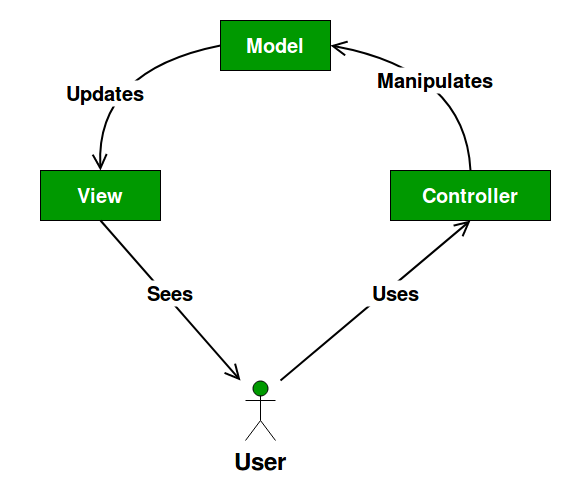
\includegraphics[scale=0.4]{pictures/mvc.png}
    \caption{MVC pattern visualized, source: \href{https://pushkarbaichwal7937.medium.com/model-view-controller-in-java-e57b1f754c9e}{Pushar Baichwal}}
    \label{mvcExample}
\end{figure}
\par
The Model concern represents the data and business logic of the application.
It encapsulates the application's data and the access to the said data.
It is tightly coupled with the View concern, as it notifies it for any changes in data.
\par
The View concern deals with the UI (User Interface) of our application.
Its role is to display the data and handle user interactions.
Because of this, it is tightly coupled to the Controller concern.
\par
The Controller concern is used as a connecting piece between the View and the Model concerns.
It is the layer that interprets the user input and makes calls to the model objects.
Its main purpose is to update the Model and select the proper View display.


\subsection{Singleton}
Singleton is a creational design pattern that lets you ensure that the "need for one - and only one - instance of a class" \cite{singletonQ} is met.
The Singleton pattern solves two problems at the same time, violating the Single Responsibility Principle.
\begin{figure}[htbp]
    \centering
    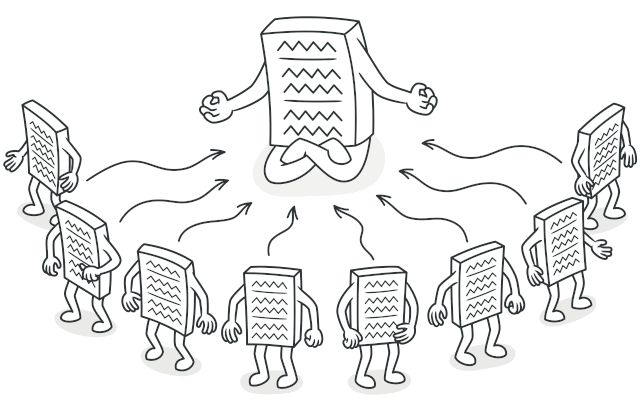
\includegraphics[scale=0.4]{pictures/singleton.png}
    \caption{Singleton pattern visualized, source: \href{https://rezababakhani.ir/blog/singleton-design-pattern}{Refactoring Guru}}
    \label{singletonExample}
\end{figure}
\par
The Singleton pattern introduces a global state, which can make it harder to track and reason about the behavior of the system.
Changes to the Singleton instance can affect other application parts, potentially resulting in hidden bugs and unintended side effects.
As the Singleton instance is directly accessed throughout the application, the use of Singleton can lead to tight coupling between classes. 
This can make it more difficult to modify or replace the Singleton in the future with a different implementation.
\par
It is worth mentioning that this pattern is great for server-side development.
Some real-world examples of the Singleton pattern include: database connections, logging, caching, thread pools, and configuration settings.
These are things that are not supposed to be instantiated more than once, as they can lead to memory leaks or other issues.
Also, due to their nature, they should not be handled in the client-side part.
\par
This is a design pattern I avoided using in the companion app, as it is not recommended for use in modern software development due to its drawbacks.
Also, because of the spawn of global state, it could result in some slowdowns in the application, as the Singleton instance is directly accessed throughout the application.


\subsection{MVVM}
\par
MVVM is a design pattern that separates into the following concerns: the Model, the View, and the ViewModel. 
All the concerns have their own responsibility and are specific handlers for some use cases.
This design pattern is considered one of the best, as "regardless of how you implement the pattern, doing so is good practice" \cite{mvvmQ}.
Below we will take a look at each concern and see how it is implemented in the companion app.
This design pattern is used in almost all cross-platform frameworks to provide a clear separation between the application logic and the user interface.
\begin{figure}[htbp]
    \centering
    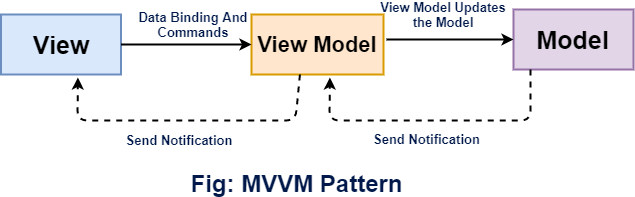
\includegraphics[scale=0.7]{pictures/mvvm.png}
    \caption{MVVM pattern visualized, source: \href{https://www.javatpoint.com/xamarin-model-view-viewmodel-pattern}{Tutorialspoint}}
    \label{mvvmExample}
\end{figure}
\par
The Model concern represents the data and business logic of the application. 
It encapsulates the application's data and the rules that govern access to and updates of this data. 
It is responsible for fetching data from the database or any other data source, and it ensures that the data is valid. 
This is notable in the companion app as well, by providing \textit{Service} and \textit{Provider} layers, 
each being themselves separated into units that are responsible for handling the functionality of a single entity.
\begin{figure}[htbp]
    \centering
    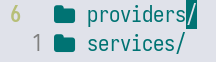
\includegraphics[scale=1.0]{pictures/service_provider.png}
    \caption{Service and Provider layers (Model concern)}
    \label{serviceProviderExample}
\end{figure}
\par
The View concern deals with the UI (User Interface) of our application. 
Its role is to display the data and handle user interactions, by sending them to the ViewModel concern. 
This is observable in the companion app through widget trees.
\begin{figure}[htbp]
    \centering
    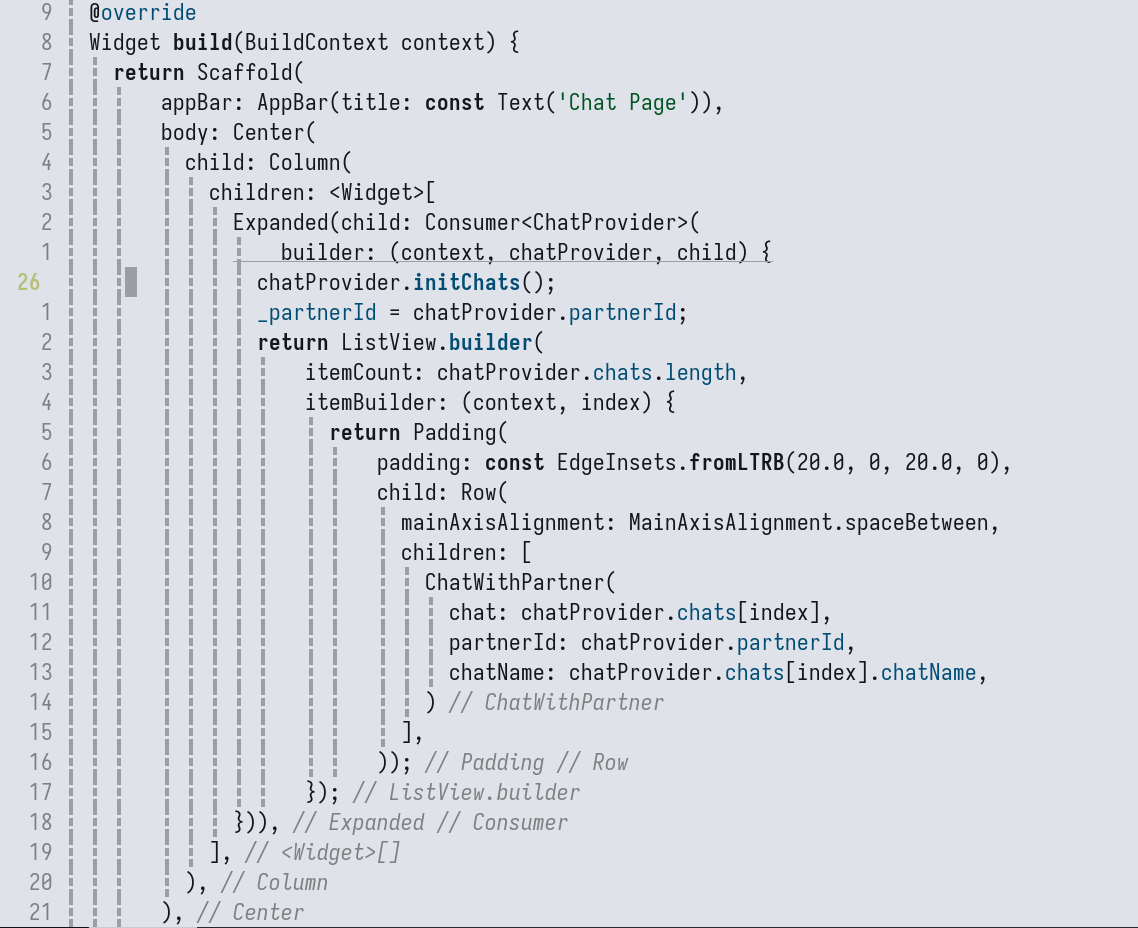
\includegraphics[scale=0.3]{pictures/widget_tree.png}
    \caption{Widget tree (View concern)}
    \label{widgetTreeExample}
\end{figure}
\par
The ViewModel is the liant between the View and the Model concerns, as the name suggests. 
Its primary role is to update the Model based on the inputted user interactions. 
It is usually the concern that handles state management, but since our companion app is mostly stateless, 
this turns our \textit{Provider} layer into a ViewModel concern handler.

\par
Data binding is a key feature of MVVM that allows automatic synchronization of data between the View and ViewModel. 
Changes in the ViewModel are automatically reflected in the View and vice versa. Most of the current cross-platform frameworks have a built-in data binder, 
so there is almost no need to build it. 
This is important, because it means that less code needs maintenance, due to the framework's maintenance being done internally.

\subsection{Observer}
\par
The Observer design pattern is a behavioral design pattern that defines a one-to-many dependency between objects so that when one object changes state, 
all its dependents are notified and updated automatically. 
It was first codified by "a group of IBM researchers" \cite{observerDesignPattern} in the 1994 book Design Patterns.
It is used to establish a subscription mechanism to allow multiple objects (\textit{Observers}) to listen and react to events or changes in another object (\textit{Subject}).
\begin{figure}[htbp]
    \centering
    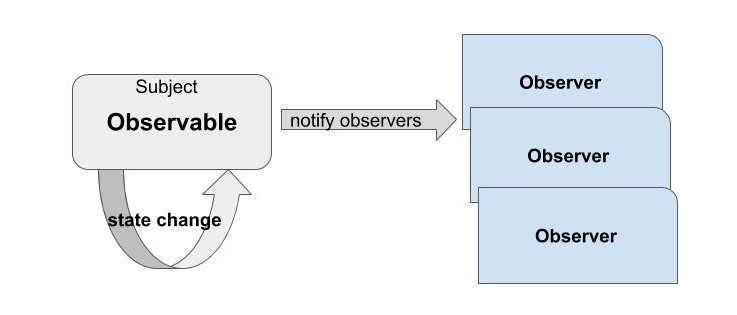
\includegraphics[scale=0.4]{pictures/observer.jpg}
    \caption{Observer pattern visualized, source: \href{https://gustavopeiretti.com/observer-design-pattern/}{Gustavo Peiretti}}
    \label{observerExample}
\end{figure}
\par
The Observer defines a one-to-many relationship between objects so that when one object changes state, all its dependents are notified and updated automatically.
This is useful for building loosely coupled systems, where objects can interact without having direct references to each other.
The Observer pattern is commonly used in event-driven programming, where objects can subscribe to events and receive notifications when the events occur.
It is a good fit for separating concerns, as it provides a clear separation between the object that generates events and the objects that react to the events.
\par
The Observer pattern is also used in the companion app to notify the UI when the data changes.
This is done by using the \textit{Provider} layer, which is a state management solution that allows the UI to listen for changes in the data and update accordingly.
This turns the Provider object into a Subject, and all the notified objects into Observers.
Such an implementation of the Observer allows for a responsive, and most importantly "stateless" UI, 
in the sense that traditional "states" (such as the ones in React or Flutter) are not being used, due to them being runtime heavy.
\begin{figure}[htbp]
    \centering
    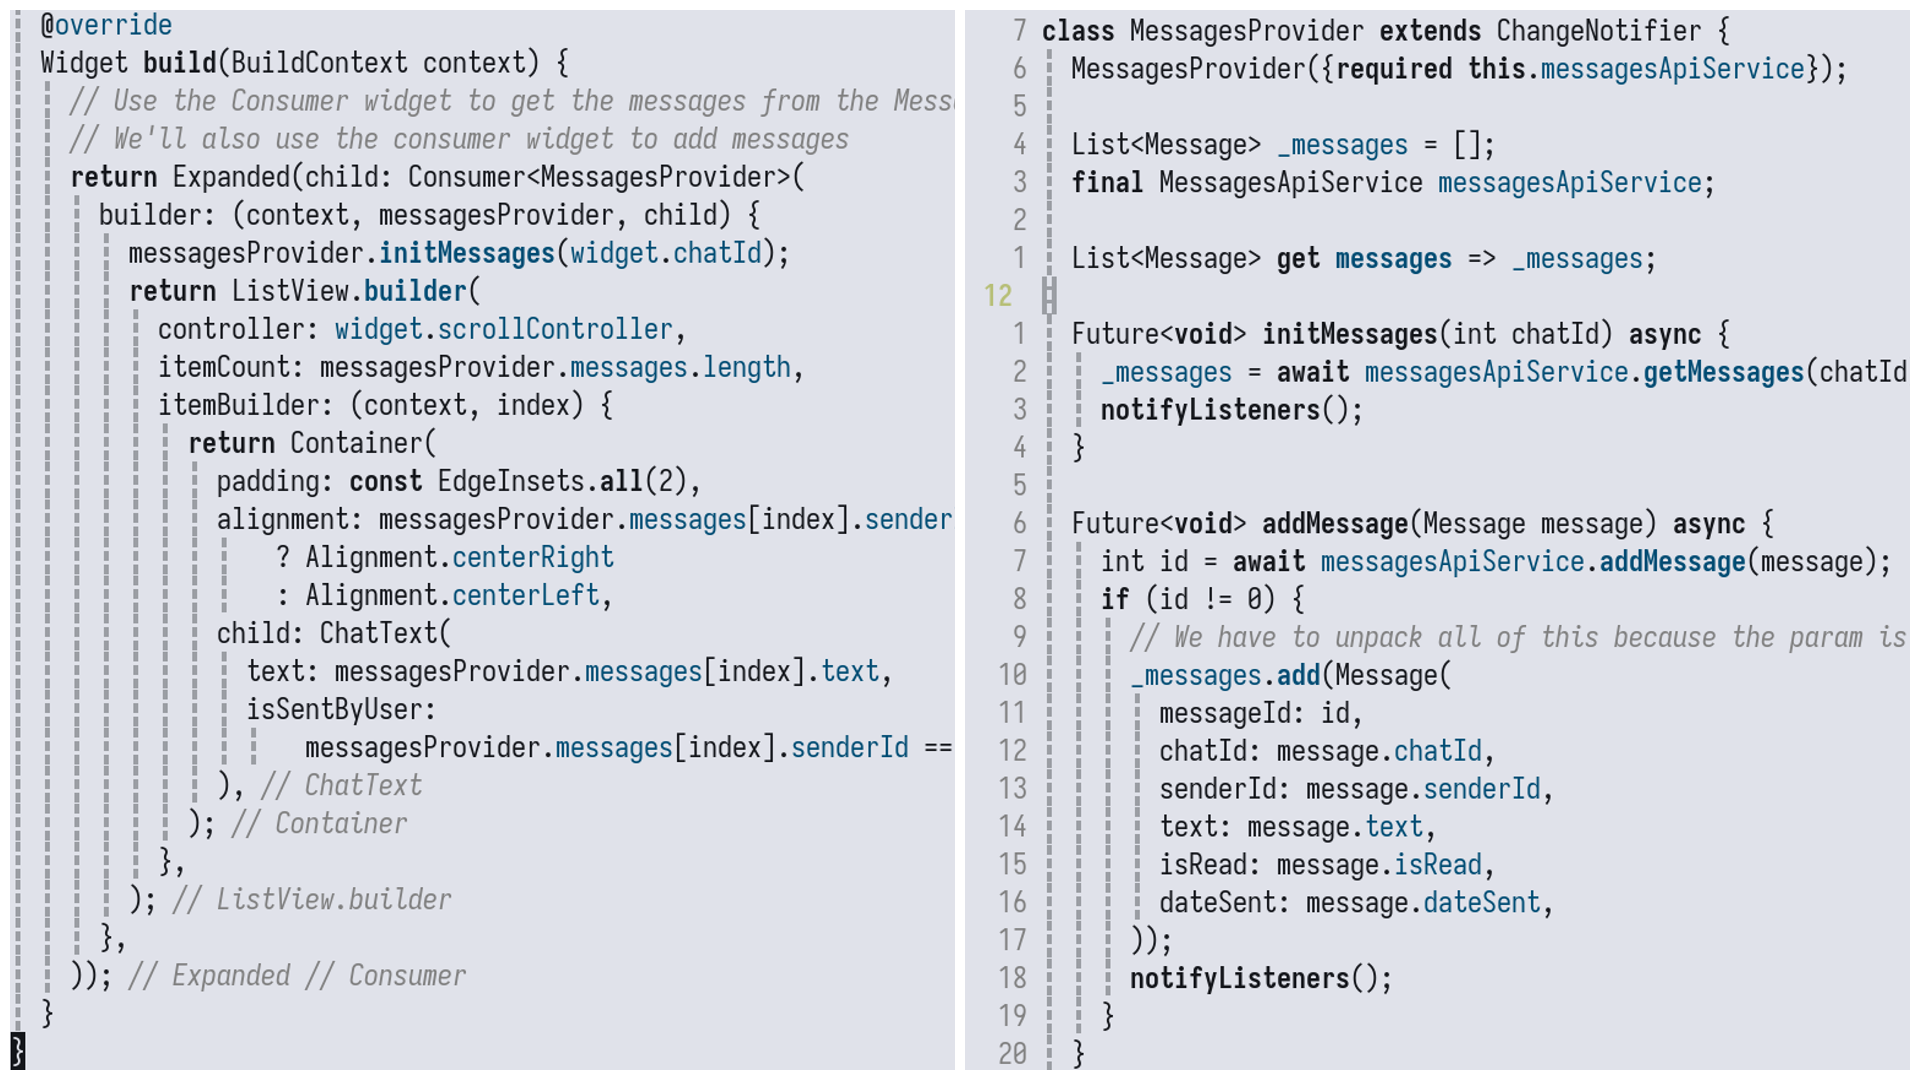
\includegraphics[scale=0.23]{pictures/subject_observer.png}
    \caption{Consumer/Observer on left, and Provider/Subject on right}
    \label{subjectObserverExample}
\end{figure}

\par
The Observer pattern is a good fit for building cross-platform applications, as it provides a flexible and scalable way to manage dependencies between objects.
The MVVM design pattern follows, in a way, the Observer pattern, as the ViewModel concern acts as an Observer that listens for changes in the Model and updates the View accordingly.
This is a good example of how the Observer pattern can be used to create a responsive and interactive user interface in a cross-platform application.
Also, with it, we can achieve a good separation of concerns, as the ViewModel concern is responsible for updating the Model based on the user interactions, 
and the View concern is responsible for displaying the data and handling user interactions.



\section{Tools}
By tools, we refer to the software and libraries that are used in cross-platform development.
This includes frameworks, libraries, and development environments that help streamline the development process and provide essential functionality for building cross-platform applications.
Here are some of the most popular tools used in cross-platform development today.

\subsection{Flutter}
Flutter is an open-source UI toolkit for building natively compiled applications for mobile, web, and desktop from a single codebase.
It provides a rich set of pre-built components and tools that can be used to create responsive and interactive user interfaces.
This enables Flutter to stick to the "write once, deploy everywhere" \cite{flutterQ} paradigm.
Flutter uses the Dart programming language, which is designed for building modern, object-oriented applications.
It also provides a hot reload feature that allows developers to quickly see changes to the code reflected in the application without restarting the app.
It is a popular choice for building cross-platform applications due to its ease of use, performance, and flexibility.
By being very easily adaptable to the separation of concerns principle, as it provides a clear separation between the application logic and the user interface, this would be a good choice for a cross-platform development tool, hence the use of this tool for the case study.
Distinct features of Flutter include:
\begin{itemize}
    \item Hot reload
    \item Rich set of pre-built components
    \item Support for mobile, web, and desktop platforms
    \item Dart programming language, designed for building modern, object-oriented applications, and also very easy to learn.
\end{itemize}

\subsection{React Native}
React Native is an open-source framework for building natively compiled applications for mobile devices from a single codebase.
It is also performant, run time wise, due to its "asynchronous calls to the underlying mobile OS" \cite{reactNativeQ}.
It uses the React JavaScript library to create user interfaces and provides a rich set of pre-built components and tools for building cross-platform applications.
React Native is a popular choice for building mobile applications due to its ease of use, performance, and flexibility.
It also provides the hot reload feature aforementioned. 
React Native is a good choice for building cross-platform applications due to its support for a wide range of platforms and devices.

\subsection{Xamarin}
Xamarin is an open-source framework for building natively compiled applications for mobile devices from a single codebase.
It is a descendant of the "open source Mono Project that brought .NET to Linux" \cite{xamarinQ}.
It uses the C\# programming language and the .NET framework to create cross-platform applications.
Xamarin provides a rich set of pre-built components and tools for building mobile applications, including support for iOS, Android, and Windows devices.
It also provides a hot reload feature that allows developers to quickly see changes to the code reflected in the application without restarting the app.


\label{chap:ch4}
